
\phantomsection


\chapter{Metodologia do projeto}\label{cap:Metodologia do projeto}

O presente capítulo mostra a metodologia e as etapas realizadas para o projeto do dispositivo desenvolvido.

\section{Modelo PRODIP}

O projeto de um produto engloba todas as etapas de definição das funções e características operacionais necessárias em um produto a ser desenvolvido, o modelo PRODIP divide o projeto em macro etapas, cada uma contemplando uma fase do desenvolvimento de um produto, conforme a \autoref{fig:Fig_401}.

\begin{figure}[htb]
	\caption{\label{fig:Fig_401}Etapas da metodologia PRODIP}
	\begin{center}
		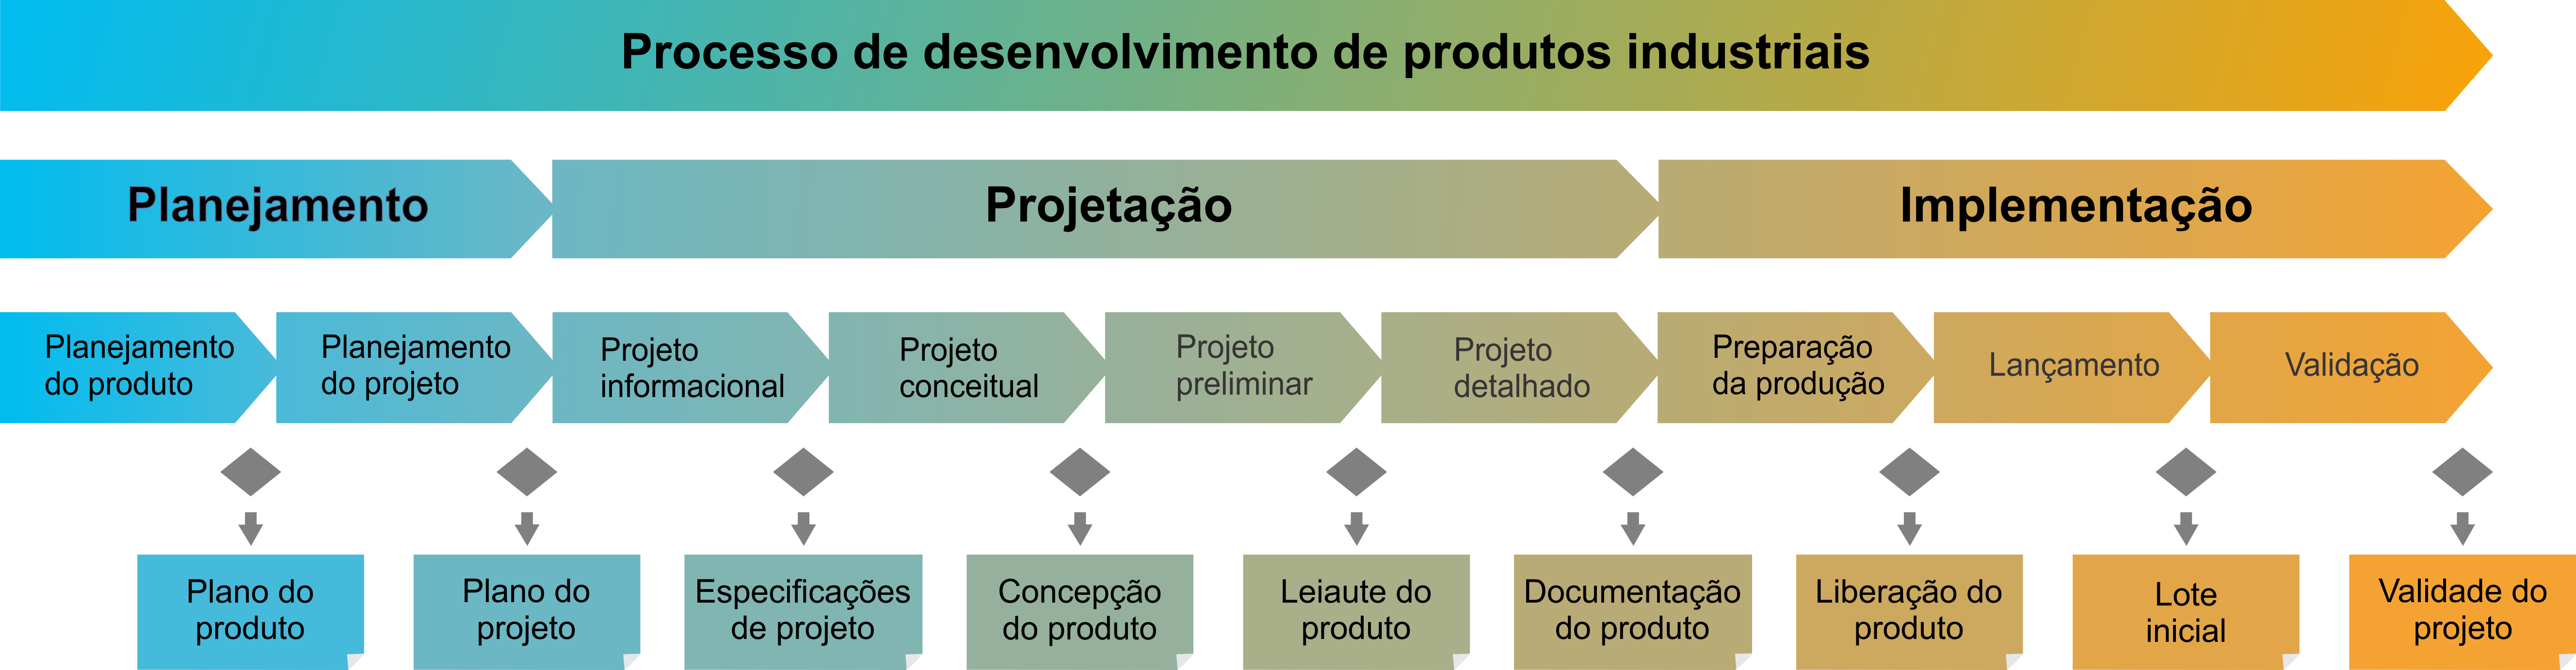
\includegraphics[width=\textwidth]{images/img401.png}
	\end{center}
	\fonte{**PRODIP (2020)**}
\end{figure}

Essa metodologia foi utilizada para organizar e linearizar as atividades de desenvolvimento do dispositivo, certas etapas ilustradas foram ignoradas e outras adicionadas devido ao objetivo do projeto e o tipo do produto desenvolvido.

\subsection{Fase de planejamento}

A fase de planejamento do projeto visa definir as etapas de desenvolvimento das ideias selecionadas utilizando definições de escopo, cronograma, orçamento riscos etc. Nessa etapa são definidas as ideias do problema e produto, então é feito um mapeamento tecnológico, em que, segundo a metodologia "são organizadas as informações do mercado, produto e tecnologia ao longo do tempo. Essas informações são correlacionadas e servem de base para estabelecer o plano de produtos." (PRODIP, 2020).

O problema proposto foi o de encontrar a solução para a medição de torque dinâmico em aplicações automotivas, e a principal motivação é o fato de que foi verificado ser um tipo de grandeza não muito monitorada devido a dificuldade de obtenção dos valores e do custo, peso e complexidade dos dispositivos existentes para esses fins atualmente. Os principais tipos de produtos disponíveis identificados para esse tipo de aplicação são os transdutores de torque, utilizados em ramos industriais, e os dinamômetros de bancada, que são usualmente utilizados para identificar as curvas de torque e potência de motores.

Os transdutores de torque são de maior interesse dado o princípio de funcionamento, segundo a fabricante Kyowa  (%https://www.kyowa-ei.com/eng/technical/sensors/torque.html
acesso em julho de 2020) seus transdutores de torque convertem torção, calculadas pela tensão de cisalhamento superficial, em tensão elétrica, garantem medição fácil e acurada de torque sob condições de funcionamento desde paradas até altas rotações, e devido ao fato de serem utilizados extensômetros como sensor, medidas estáveis e precisas são garantidas até em longas durações de operação e condições severas. A \autoref{fig:Fig_403} mostra os principais componentes desse tipo de dispositivo.

\begin{figure}[htb]
	\caption{\label{fig:Fig_403}Principais componentes de um transdutor de torque industrial}
	\begin{center}
		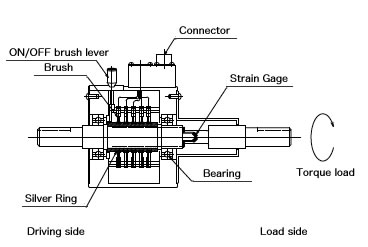
\includegraphics{images/img403.jpg}
	\end{center}
	\fonte{**Showa Sokki (acesso em julho de 2020)
		%http://www.showa-sokki.co.jp/English/Products_e/Torque_Tr_e.html%
		**}
\end{figure}

**falar que o principio de funcionamento do transdutor de torque é a principal influência para a escolha das palavras chave da revisão bibliográfica**

%O princípio de funcionamento dos transdutores industriais é baseado na leitura das tensões superficiais de um eixo utilizando extensômetros, foi definido que o principio de funcionamento do dispositivo seguiria os mesmos princípios ja utilizados, então foi feita a revisão bibliográfica (detalhada no capítulo 2).

Com os dados do mapeamento tecnológico e da revisão dos trabalhos científicos recentes, é elaborado um escopo base do projeto, seguido pela definição de um conceito básico de funcionamento, os componentes necessários e os respectivos preços, estes dados estão disponíveis no apêndice A. (**Falta anexar, arquivo 0 - Escopo do projeto no drive, planilha "mapa de tecnologias", incorporar uma parte da planilha de revisão bibliográfica junto**)

\subsection{Projeto Informacional}

O projeto informacional utiliza ferramentas para definição de especificações de projeto que irão orientar o desenvolvimento do produto, o principal é a matriz QFD, utilizada para definir a importância dos requisitos do produto.

\begin{figure}[htb]
	\caption{\label{fig:Fig_401}Etapas do projeto informacional}
	\begin{center}
		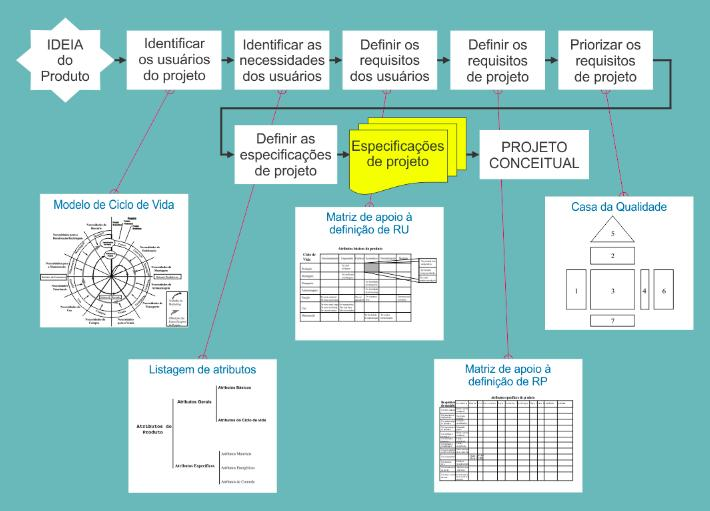
\includegraphics[width=\textwidth]{images/img402.jpg}
	\end{center}
	\fonte{**PRODIP (2020)**}
\end{figure}

-realizar as pesquisas de mercado, listagem de atributos e desenvolver a matriz QFD.

\subsection{Projeto Conceitual}

Busca de soluções conceituais para o problema, onde as alternativas são geradas e avaliadas técnica e economicamente, as ferramentas disponíveis são a síntese de funções, matriz morfológica e matriz multi critério de seleção

%\subsection{Projeto Preliminar}
%
%“Solução conceitual é desenvolvida em termos de layout, arranjo, formas, geometria, materiais e processos de fabricação”. A configuração da solução solucionada (embodiment design). modelos de análise, simulação e otimização da solução são empregados. Construção e testes de protótipos.
%
%\subsection{Projeto Detalhado}
%
%Os detalhes da solução otimizada são finalizados. Concluem-se os testes de protótipos e revisa-se a solução em detalhes, prepara-se a documentação final do produto e da produção
